% Chapter Template

\chapter{Visualizaciones} % Main chapter title

\label{VISUALIZACIÓN} % Change X to a consecutive number; for referencing this chapter elsewhere, use \ref{ChapterX}

%----------------------------------------------------------------------------------------
%	SECTION 1
%----------------------------------------------------------------------------------------

\section{Representaciones clásicas del mutualismo}

Las visualizaciones son una herramienta cada día más importante en el análisis de la información, y en particular en la ciencia de redes. La representación gráfica resulta fundamental en el análisis exploratorio pero también para la síntesis de los resultados. Para redes ecológicas se emplean gráficos de uso común en la representación de redes sociales \cite{freeman2012social}. Quizá porque su tamaño es reducido en comparación con otras aplicaciones, no ha habido apenas desarrollo de herramientas y gráficas específicas para este campo de aplicación \cite{yoon20043d, kazanci2007econet}.

En el análisis del mutualismo se utilizan de forma reiterada dos representaciones: el diagrama bipartito y la matriz de interacción. Ambas  son sencillas y ponen de manifiesto la separación entre clases de especies, pero tienen inconvenientes importantes. 

En el diagrama bipartito se disponen las especies en dos filas paralelas, ya sean horizontales o verticales
y se unen aquellas que interactúan.

\begin{figure}[h!]
\centering
\includegraphics[scale=0.33]{Figures/VIS_bipartito_SD_001.png}
\caption{Diagrama bipartito de una red de dispersores en New Jersey \cite{baird1980selection}.}
\label{fig:VIS_bipartito_SD_001}
\end{figure}

En el ejemplo de la figura \ref{fig:VIS_bipartito_SD_001} la red es de un tamaño reducido, puede distinguirse el núcleo de plantas más conectadas (de la $1$ a la $4$ y los enlaces se ven con claridad. Cuando el número de especies supera unas pocas decenas, la situación cambia de forma radical.

\begin{figure}[h!]
\centering
\includegraphics[scale=0.4]{Figures/VIS_bipartito_SD_020.png}
\caption{Red de dispersores en Nava Correhuelas, Sierra de Cazorla, España. Compilada por Pedro Jordano, no publicada.}
\label{fig:VIS_bipartito_SD_020}
\end{figure}

La red de la figura \ref{fig:VIS_bipartito_SD_020} tiene $58$ especies y $150$ enlaces, frente a $28$ especies y $50$ enlaces de la anterior. Es una red de dimensiones moderadas, pero ya es muy complicado seguir los detalles del gráfico. A pesar de ello, algunos autores consiguen resultados excelentes con redes de dimensiones similares a las de este segundo ejemplo, jugando con formas, colores y tamaños \cite{dakos2014critical}. Cuando se llega al centenar de especies, la zona central degenera en una mancha en la que es imposible distinguir los enlaces. Por este motivo, en la literatura sobre mutualismo solo aparecen gráficos de redes pequeñas. 

La matriz de interacción ofrece una visión más rica si los nodos se ordenan de la forma adecuada. Colocando los más conectados en la parte superior izquierda, es fácil localizar el núcleo de especies generalistas. Con redes pequeñas como la del primer ejemplo, el resultado es muy satisfactorio.

\begin{figure}[h!]
\centering
\includegraphics[scale=0.4]{Figures/VIS_matrix_SD_001.png}
\caption{Matriz de interacción de una red de dispersores en New Jersey \cite{baird1980selection}. Las casillas coloreadas indican la existencia de enlace.}
\label{fig:VIS_matrix_SD_001}
\end{figure}

Por el contrario, la matriz de interacción pierde gran parte de su utilidad para redes grandes, como muestra la figura \ref{fig:VIS_matrix_PL_001}.

\begin{figure}[h!]
\centering
\includegraphics[scale=0.4]{Figures/VIS_matrix_PL_001.png}
\caption{Matriz de interacción de una red de polinizadores en Los Andes, Chile \cite{arroyo1982community}.}
\label{fig:VIS_matrix_PL_001}
\end{figure}

A continuación se describen dos nuevos tipos de visualización que se basan en las \textit{k magnitudes} definidas en el capítulo anterior. Se han diseñado para resolver los problemas descritos en este apartado introductorio.

\section{Visualizaciones basadas en \textit{k-magnitudes}}


\subsection{El diagrama polar}

Nunc posuere quam at lectus tristique eu ultrices augue venenatis. Vestibulum ante ipsum primis in faucibus orci luctus et ultrices posuere cubilia Curae; Aliquam erat volutpat. Vivamus sodales tortor eget quam adipiscing in vulputate ante ullamcorper. Sed eros ante, lacinia et sollicitudin et, aliquam sit amet augue. In hac habitasse platea dictumst.

\begin{figure}[h!]
\centering
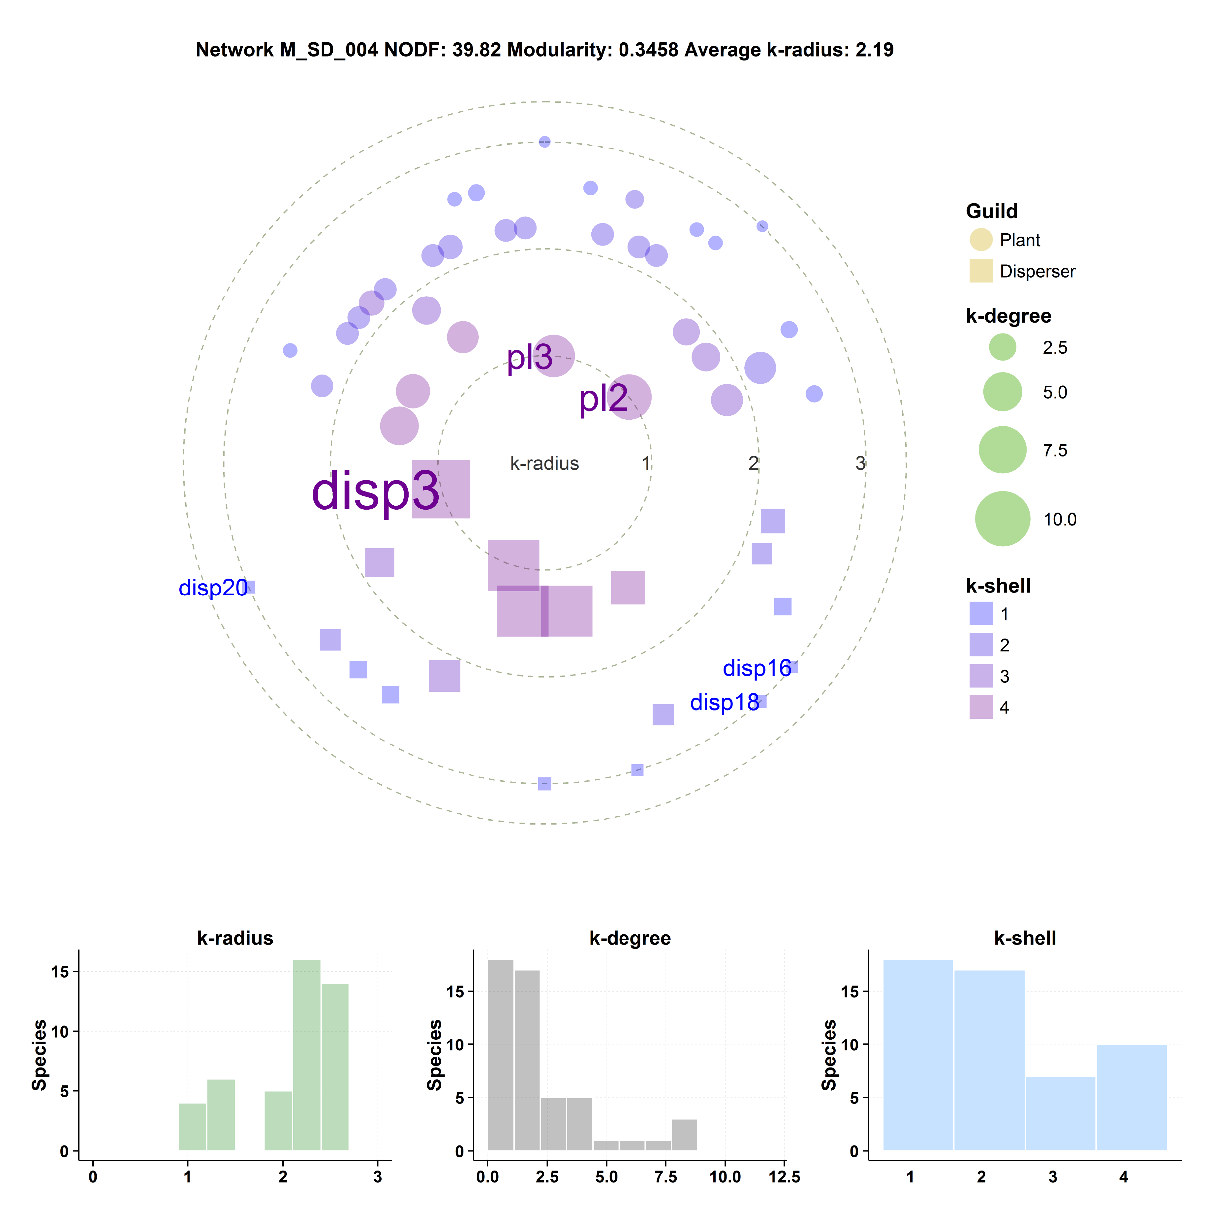
\includegraphics[scale=0.6]{Figures/M_SD_004_polar.eps}
\caption[PolarExample]{Ejemplo de diagrama polar.}
\label{fig:polar}
\end{figure}

\subsection{El diagrama zigurat}

Nunc posuere quam at lectus tristique eu ultrices augue venenatis. Vestibulum ante ipsum primis in faucibus orci luctus et ultrices posuere cubilia Curae; Aliquam erat volutpat. Vivamus sodales tortor eget quam adipiscing in vulputate ante ullamcorper. Sed eros ante, lacinia et sollicitudin et, aliquam sit amet augue. In hac habitasse platea dictumst.

\begin{figure}[h!]
\centering
\includegraphics[scale=0.5]{Figures/zig_pl_024.png}
\caption[PolarExample]{Ejemplo de diagrama \textit{zigurat}.}
\label{fig:VISUALIZACION_zigurat}
\end{figure}

\section{Resultados}

Nunc posuere quam at lectus tristique eu ultrices augue venenatis. Vestibulum ante ipsum primis in faucibus orci luctus et ultrices posuere cubilia Curae; Aliquam erat volutpat. Vivamus sodales tortor eget quam adipiscing in vulputate ante ullamcorper. Sed eros ante, lacinia et sollicitudin et, aliquam sit amet augue. In hac habitasse platea dictumst.


\section{Conclusiones}

Nunc posuere quam at lectus tristique eu ultrices augue venenatis. Vestibulum ante ipsum primis in faucibus orci luctus et ultrices posuere cubilia Curae; Aliquam erat volutpat. Vivamus sodales tortor eget quam adipiscing in vulputate ante ullamcorper. Sed eros ante, lacinia et sollicitudin et, aliquam sit amet augue. In hac habitasse platea dictumst.
